\subsection*{5.3 EXPERIMENT A: Quantification of Communication Efficiency}
\noindent The main idea behind the I.C.U.M system is the optimization of the balance between efficient and effective communication, which is what the first experiment would quantify.


\subsubsection*{Methodology}
\noindent Performance accuracy was evaluated using \textbf{On-Device RMSE}. It is important to clarify that this metric validates the \textit{internal belief} of the distributed swarm, operating purely on local neighbor distances. The simulator acts as an "Oracle" for evaluation: at each timestep, it accesses the memory of every connected node to retrieve its locally estimated coordinate $(x,y)$, and compares this entire set against the ground truth positions after rigid alignment. This approach isolates the effectiveness of the distributed positioning algorithm, ensuring that the metric reflects the system's real-time self-awareness.

\noindent The simulated environment was set up in two different states, where the Root Mean Square Error (RMSE) and total number of messages sent across the entire system were compared for 10 minutes. The first case, which we call the $baseline$, acts as a basis for regular system operation, while the second case includes the IMU-controlled messaging, which we refer to here as $event$-$driven$ communication. By having a baseline comparison, we would be able to directly measure the impact of event-driven communication on the error in location data, to see if efficient communication would have a negative effect on the overall location accuracy. \\
Figures \ref{fig:A_RSME} and \ref{fig:A_Tx} below illustrate the RSME at the different points in time and the number of messages sent during this experiment.

\begin{figure}[h] %float with two figures
\centering
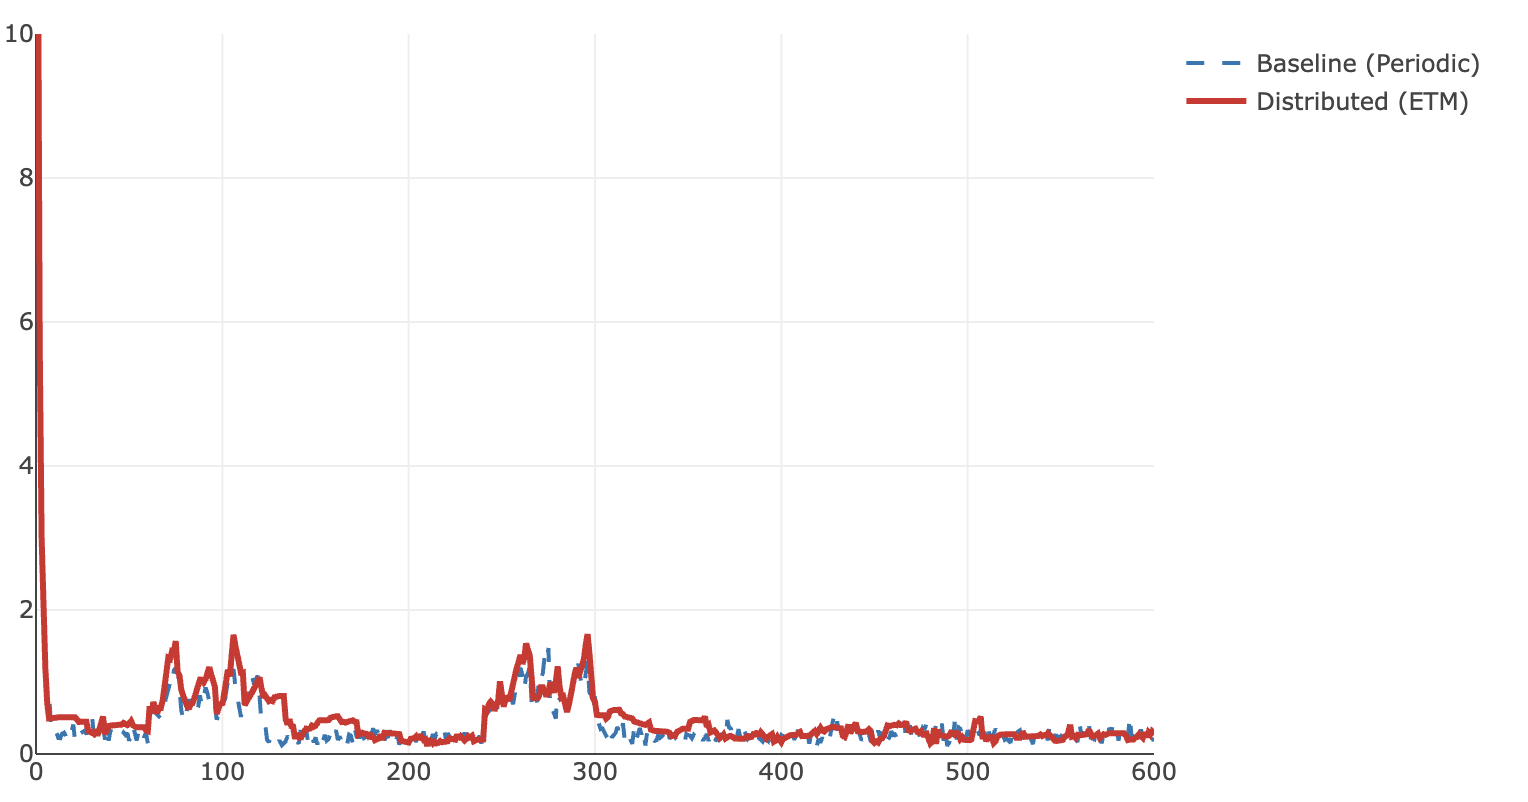
\includegraphics[width= 1\linewidth]{images'nshi/exp_a/A_50_moving_01_noise.png}
\caption{Graph depicting the Aligned Root Mean Square Error ($y$-$axis$) over time ($x$-$axis$). The blue line is the baseline, while the red line is with event-driven communication \label{fig:A_RSME}}\bigskip 
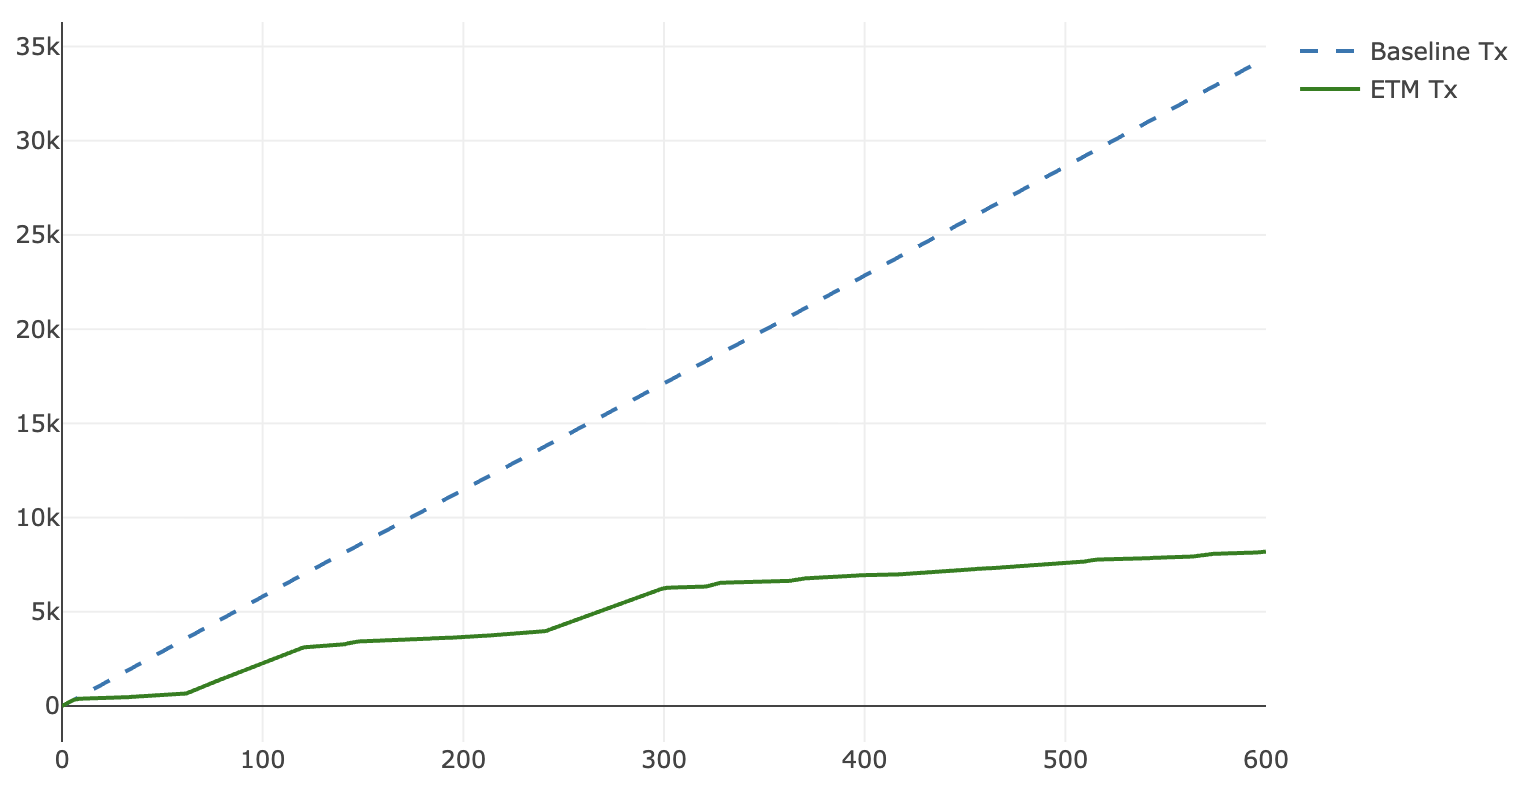
\includegraphics[width= 1\linewidth]{images'nshi/exp_a/a_50_moving_01_noise_msg_total.png}
\caption{Graph depicting the amount of messages ($y$-$axis$) over time ($x$-$axis$). The blue dotted line is the baseline, while the green line is with event-driven communication \label{fig:A_Tx}}
\end{figure}
\noindent While the RMSE is largely the same for both cases, the message rate for the latter sees a significant reduction. At 600 seconds, the number of messages sent is $34,390$ and $8,195$ respectively, which is an $76.17\%$ decrease in the number of messages sent for the event-driven case. We argue that the difference in RMSE is insignificant when compared to the staggering decrease in messages sent, which undoubtedly positively impacts the system's battery performance and expected lifetime. To measure this, we would need to know exactly how much power the nodes spend on messaging. With only a novel system, actual testing of hardware becomes difficult. We will instead illustrate power saving as bounded estimates.
\noindent If we assume that BLE power consumption scales linearly, we can derive the battery life as follows, where $L$ is the total battery life, $B$ is the total battery capacity, and $P$ is the power spent
\begin{equation}
    L = \frac{B}{P}
\end{equation}
$P$ can be split into two variables, one for the power consumed by BLE and one for the rest of the node's computational tasks
\begin{equation}
    P_{total}=P_{BLE}+P_{other}
\end{equation}
The power spent on BLE messaging can be defined as
\begin{equation}
    P_{BLE} = E\times P_{total}
\end{equation}
where $E$ is the energy percentage that BLE uses, and if we take the reduced messaging rate of $76.17\%$, we get a new BLE power consumption
\begin{equation}
    P_{BLE, New} = (1-0.7617)\times P_{BLE}
\end{equation}
\begin{equation}
    P_{BLE, New} = (1-0.7617) \times E \times P_{total}
\end{equation}
The power that the system additionally uses can be redefined as
\begin{equation}
    P_{other, new}=P_{total}-P_{BLE, new}
\end{equation}
\begin{equation}
    P_{other, new}=P_{total}-E\times P_{total}
\end{equation}
\begin{equation}
    P_{other, new}=(1-E)\times P_{total}
\end{equation}
From this, we can derive the formula for the new power consumption
\begin{equation}
    P_{total, new} = P_{other,new}+ P_{BLE, new}
\end{equation}
\begin{equation}
    P_{total, new} = (1-E)\times P_{total}+ (1-0.7617) \times E \times P_{total}
\end{equation}
\begin{equation}
    P_{total, new} = P_{total}[(1-E)+ (1-0.7617) \times E]
\end{equation}
\begin{equation}
    P_{total, new} = P_{total}(1-0.7617E)
\end{equation}
Subsequently, the formula for computing the new battery life becomes
\begin{equation}
    L_{new} = \frac{B}{P_{total, new}} = \frac{B}{ P_{total}(1-0.7617E)}
\end{equation}
Assuming ideal conditions, where battery capacity $B$ is $1$, while the starting battery percentage $P_{total, new}$ is also $1$, the final formula that we will use to compute the bounds becomes
\begin{equation}
  \frac{1}{(1-0.7617E)}
\end{equation}
Again, we cannot verify what percentage of battery life is used for BLE messaging, but we can compute upper and lower bounds on the battery-life improvement. Figure \ref{fig:battery} shows, after 10 minutes, the percentage improvement in battery life ($y$-$axis$) as a function of $E$, the total battery percentage devoted to BLE messaging at $5\%$ intervals($x$-$axis$).
\begin{figure}[H] %float with two figures
\centering
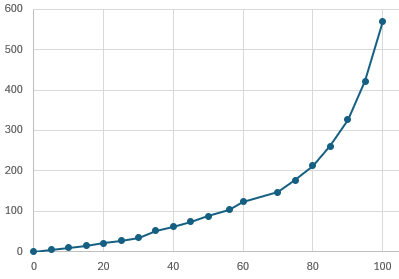
\includegraphics[width= 1\linewidth]{images'nshi/battery savings.PNG}
\caption{Graph depicting the percentage improvement in battery life ($y$-$axis$) when the battery consumption of BLE messaging is at different percentages ($x$-$axis$) \label{fig:battery}}
\end{figure}
\noindent Any reduction in BLE messaging results in an increase in battery life, though the achievable improvement varies exponentially depending on how dominant BLE communication is in the overall energy budget. The improvements start approaching several-fold increases when BLE communication is at around $55\%$. While this is nothing concretely quantifiable, it illustrates the impact event-based communication can have on the battery life of the nodes, and by proxy, the overall system lifetime.
